%----------------------------------------------------------------------------------------
%
% A LaTeX-template for 1DV510. Modified and translated by Björn Lindenberg at LNU.
% Based on an original master thesis template created by Marcus Wilhelmsson at LNU.
%
%----------------------------------------------------------------------------------------

% Settings and document configuration

\documentclass[a4paper,12pt]{article} 
\usepackage[T1]{fontenc} 
\usepackage{times} 
\usepackage[swedish,english]{babel} 
\usepackage[utf8]{inputenc} 
\usepackage{dtk-logos} 
\usepackage{wallpaper} 
\usepackage[absolute]{textpos} 
\usepackage[top=2cm, bottom=2.5cm, left=3cm, right=3cm]{geometry} 
\usepackage[parfill]{parskip} 
\usepackage{csquotes} 
\usepackage{float} 
\usepackage{lipsum} % Used for dummy text. Can be removed.
\usepackage{listings, color}
\lstdefinestyle{Asm}{
  belowcaptionskip=1\baselineskip,
  breaklines=true,
  frame=L,
  xleftmargin=\parindent,
  language=[x86masm]Assembler,
  showstringspaces=false,
  basicstyle=\footnotesize\ttfamily,
  keywordstyle=\bfseries\color{purple!40!black},
  commentstyle=\itshape\color{green!40!black},
  identifierstyle=\color{blue},
  stringstyle=\color{orange},
}

% Fontsizes for section headings.
\usepackage{sectsty} 
\sectionfont{\fontsize{14}{15}\selectfont}
\subsectionfont{\fontsize{12}{15}\selectfont}
\subsubsectionfont{\fontsize{12}{15}\selectfont}

%----------------------------------------------------------------------------------------
%	This part is used for the text box on the title page
%----------------------------------------------------------------------------------------
\newsavebox{\mybox}
\newlength{\mydepth}
\newlength{\myheight}

\newenvironment{sidebar}%
{\begin{lrbox}{\mybox}\begin{minipage}{\textwidth}}%
{\end{minipage}\end{lrbox}%
 \settodepth{\mydepth}{\usebox{\mybox}}%
 \settoheight{\myheight}{\usebox{\mybox}}%
 \addtolength{\myheight}{\mydepth}%
 \noindent\makebox[0pt]{\hspace{-20pt}\rule[-\mydepth]{1pt}{\myheight}}%
 \usebox{\mybox}}

%----------------------------------------------------------------------------------------
%	Title
%----------------------------------------------------------------------------------------
\newcommand\BackgroundPic{
    \put(-2,-3){
    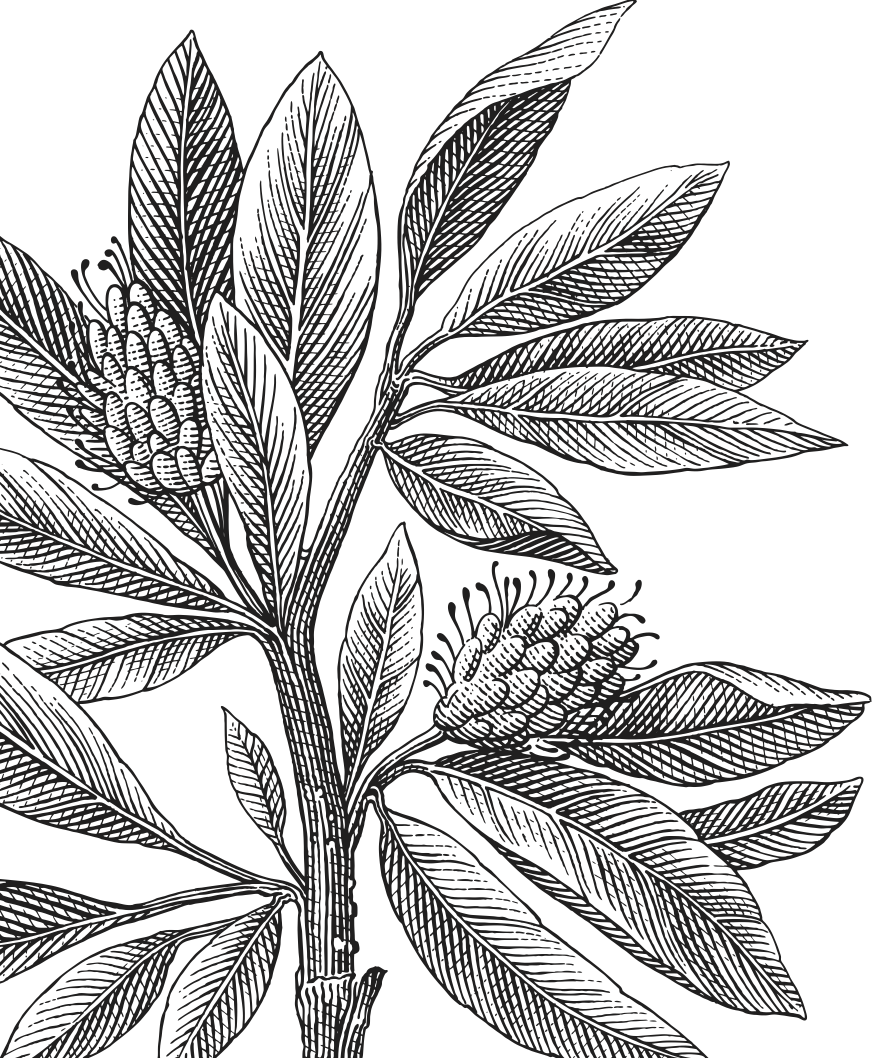
\includegraphics[keepaspectratio,scale=0.3]{img/lnu_etch.png} % Background image
    }
}
\newcommand\BackgroundPicLogo{
    \put(30,740){
    
\includegraphics[keepaspectratio,scale=0.10]{img/logo.png} % LNU logo
    }
}

\title{
\vspace{-8cm}
\begin{sidebar}
    \vspace{10cm}
    \normalfont \normalsize
    \huge Computer Technology I\\ % Main title
    \vspace{-1.3cm}
\end{sidebar}
\vspace{3cm}
\begin{flushleft}
    \huge Lab. 2 : Subroutines % Subtitle
     \small \\ \emph{}
\end{flushleft}
\null
\vfill
\begin{textblock}{5}(10,13)
\begin{flushright}
\begin{minipage}{\textwidth}
\begin{flushleft} \large
\emph{Author:}\textsc{Anas Kwefati}\\  % Author
\emph{Supervisor:}  \textsc{Anders Haggren} \\  % Author
\emph{Semester:} Autumn 2019\\ % Semester
\emph{Area:} Computer Science \\ % Area
\emph{Course code:} 1DT301 % Course
\end{flushleft}
\end{minipage}
\end{flushright}
\end{textblock}
}

\date{} % Empty date command. Use \today inside for today's date.
\author{} % Normally one would use this to define authors. However in this case the title command takes care of everything, so we leave the field empty to get rid of warnings. 

\begin{document}

\pagenumbering{gobble} % Turn off page numbering
\newgeometry{left=5cm}
\AddToShipoutPicture*{\BackgroundPic} % Adds the background image to the title page
\AddToShipoutPicture*{\BackgroundPicLogo} % Adds the logo to the title page
\maketitle % Prints the title
\restoregeometry
\clearpage

\pagenumbering{roman} % Roman page numbering for abstract page


\selectlanguage{english}

\newpage

\pagenumbering{gobble} % Turn off page numbering
\tableofcontents 

\newpage
\pagenumbering{arabic} % Turn on page numbering

%TASK1
\section{Task 1}
\lstset{style=Asm}

\begin{lstlisting}
;>>>>>>>>>>>>>>>>>>>>>>>>>>>>>>>>>>>>>>>>>>>>>>>>>>>>>>>>>>>
; 1DT301, Computer Technology I
; Date: 2016-09-15
; Author:
;	Anas Kwefati
;
; Lab number: 2
; Title: Subroutines
;
; Hardware: STK600, CPU ATmega2560
;
; Function: Program that switches between Ring counter and Johnson counter.
; 	No delay between the button is pressed and the change between Ring/Johnson.
; 	Each time I press the button, the program should change counter.

; Input ports: PORTA checks if we pressed the switch 0 (SW0; PA0).
;
; Output ports: PORTB turns on/off the light (LEDs)
;
; Subroutines: If applicable.
; Included files: m2560def.inc
;
; Other information:
;
; Changes in program: (Description and date)
;<<<<<<<<<<<<<<<<<<<<<<<<<<<<<<<<<<<<<<<<<<<<<<<<<<<<<<<<<<<

.include "m2560def.inc"

; Initialize SP, Stack Pointer
ldi r21, HIGH(RAMEND) ; R20 = high part of RAMEND address
out SPH,R21 ; SPH = high part of RAMEND address
ldi R21, low(RAMEND) ; R20 = low part of RAMEND address
out SPL,R21 ; SPL = low part of RAMEND address

;we initialize
ldi r16, 0xFF ;
out DDRB, r16 ; we set the DDRB as output

ldi r17, 0x00
out DDRA, r17 ; we set DDRA as input

ldi r16, 0xFF ; we load 0b1111 1111 to the register r16
out PORTB,r16 ; we set the PORTB to r16 SO it means that we put each light off

ldi r20, 0b11111110 ;This register will be used to check if we pressed SW0
ldi r19, 0b10111111 ;Turn on light at 0
ldi r22,0x00

loop:
	in r18, PINA ;we put the incoming data from PINA(input) to r18
	cp r20,r18 ; we compare if r20 and r18
	breq ring_counter ;if r18==r20 then go to ring_counter
	brne johnson_counter ;otherwise johnson_counter

;LED -> 0 == on and 1 == off
ring_counter:
	ldi r18, 0b11111110 ;We load 1111 1110 to r18
	call ring_loop

ring_loop:
	out PORTB, r18 ;We output r18 to PORTB, like that LED0 turns on
	call Delay ;We call the Delay
	com r18 ;we take the complement of r18. So here it would be 0000 0001
	LSL r18 ;We do a Logical Shift Left, it shifts all bits to the left.
	;So here we would get for the first r18 : 0000 0010
	com r18 ;we take the complement of r18, so we will get r18 = 1111 1101

	;Check if everything is off if true then go to ring counter to make infinite loop
	ldi r24,0xFF
	cp r24, r18 ;compare r24 with r18
	breq ring_counter ;if r24 == r18 go to ring_counter

;We check if we pressed SW0, if yes we go to Johnson_counter
	in r19, PINA
	cp r20,r19
	breq johnson_counter

	rjmp ring_loop ;we repeat the ring_loop


rjmp loop ; we go back at the beginning of the infinite loop

johnson_counter :
	ldi r19, 0b11111110 ;We load 1111 1110 to r19
	ldi r22, 0x00

johnson_loop:
	out PORTB, r19 ;We output r19 to PORTB, we turn the light LED0
	LSL r19 ; we do a logical shift left, so for the first one we will get
	; r19 = 1111 1100
	call Delay
	cp r19, r22 ;we compare r19 with r22 to check if all LEDs are turned ON
	breq johnson ;if r19==r22 then go to johnson

;Check if PINA SW0 has been pressed if yes then it goes to ring counter
	in r18, PINA
	cp r20,r18
	breq ring_counter

	rjmp johnson_loop

rjmp loop ; we go back at the beginning of the infinite loop

;We do the reverse
johnson :
	out PORTB, r22 ;Output r22 to PORTB, so all LEDs are turned ON
	ldi r22, 0b11111111 ;Load 1111 1111 to r22
	call Delay
	ldi r19,0b10000000 ; Load 1000 0000 to r19

	more_john :
		out PORTB, r19 ;Ouput r19 to PORTB, so LED7 is OFF and everything else is ON
		ASR r19 ;We do an Arithmetic Shift Right, it shifts all bits to the Right
		;So for the first one it will be r19 = 1100 0000
		call Delay
		cp r19, r22 ;compare r19 and r22
		breq johnson_counter ; if r19 == r22 go to johnson_counter to repeat the process

;Check if PINA SW0 has been pressed if yes then it goes to ring counter
		in r18, PINA
		cp r20,r18
		breq ring_counter

	rjmp more_john



Delay :
; Generated by delay loop calculator
; at http://www.bretmulvey.com/avrdelay.html

	ldi  r21, 5
    ldi  r23, 20
    ldi  r24, 175
L1: dec  r24
    brne L1
    dec  r23
    brne L1
    dec  r21
    brne L1
	ret
	
\end{lstlisting}


\begin{figure}
\begin{center}
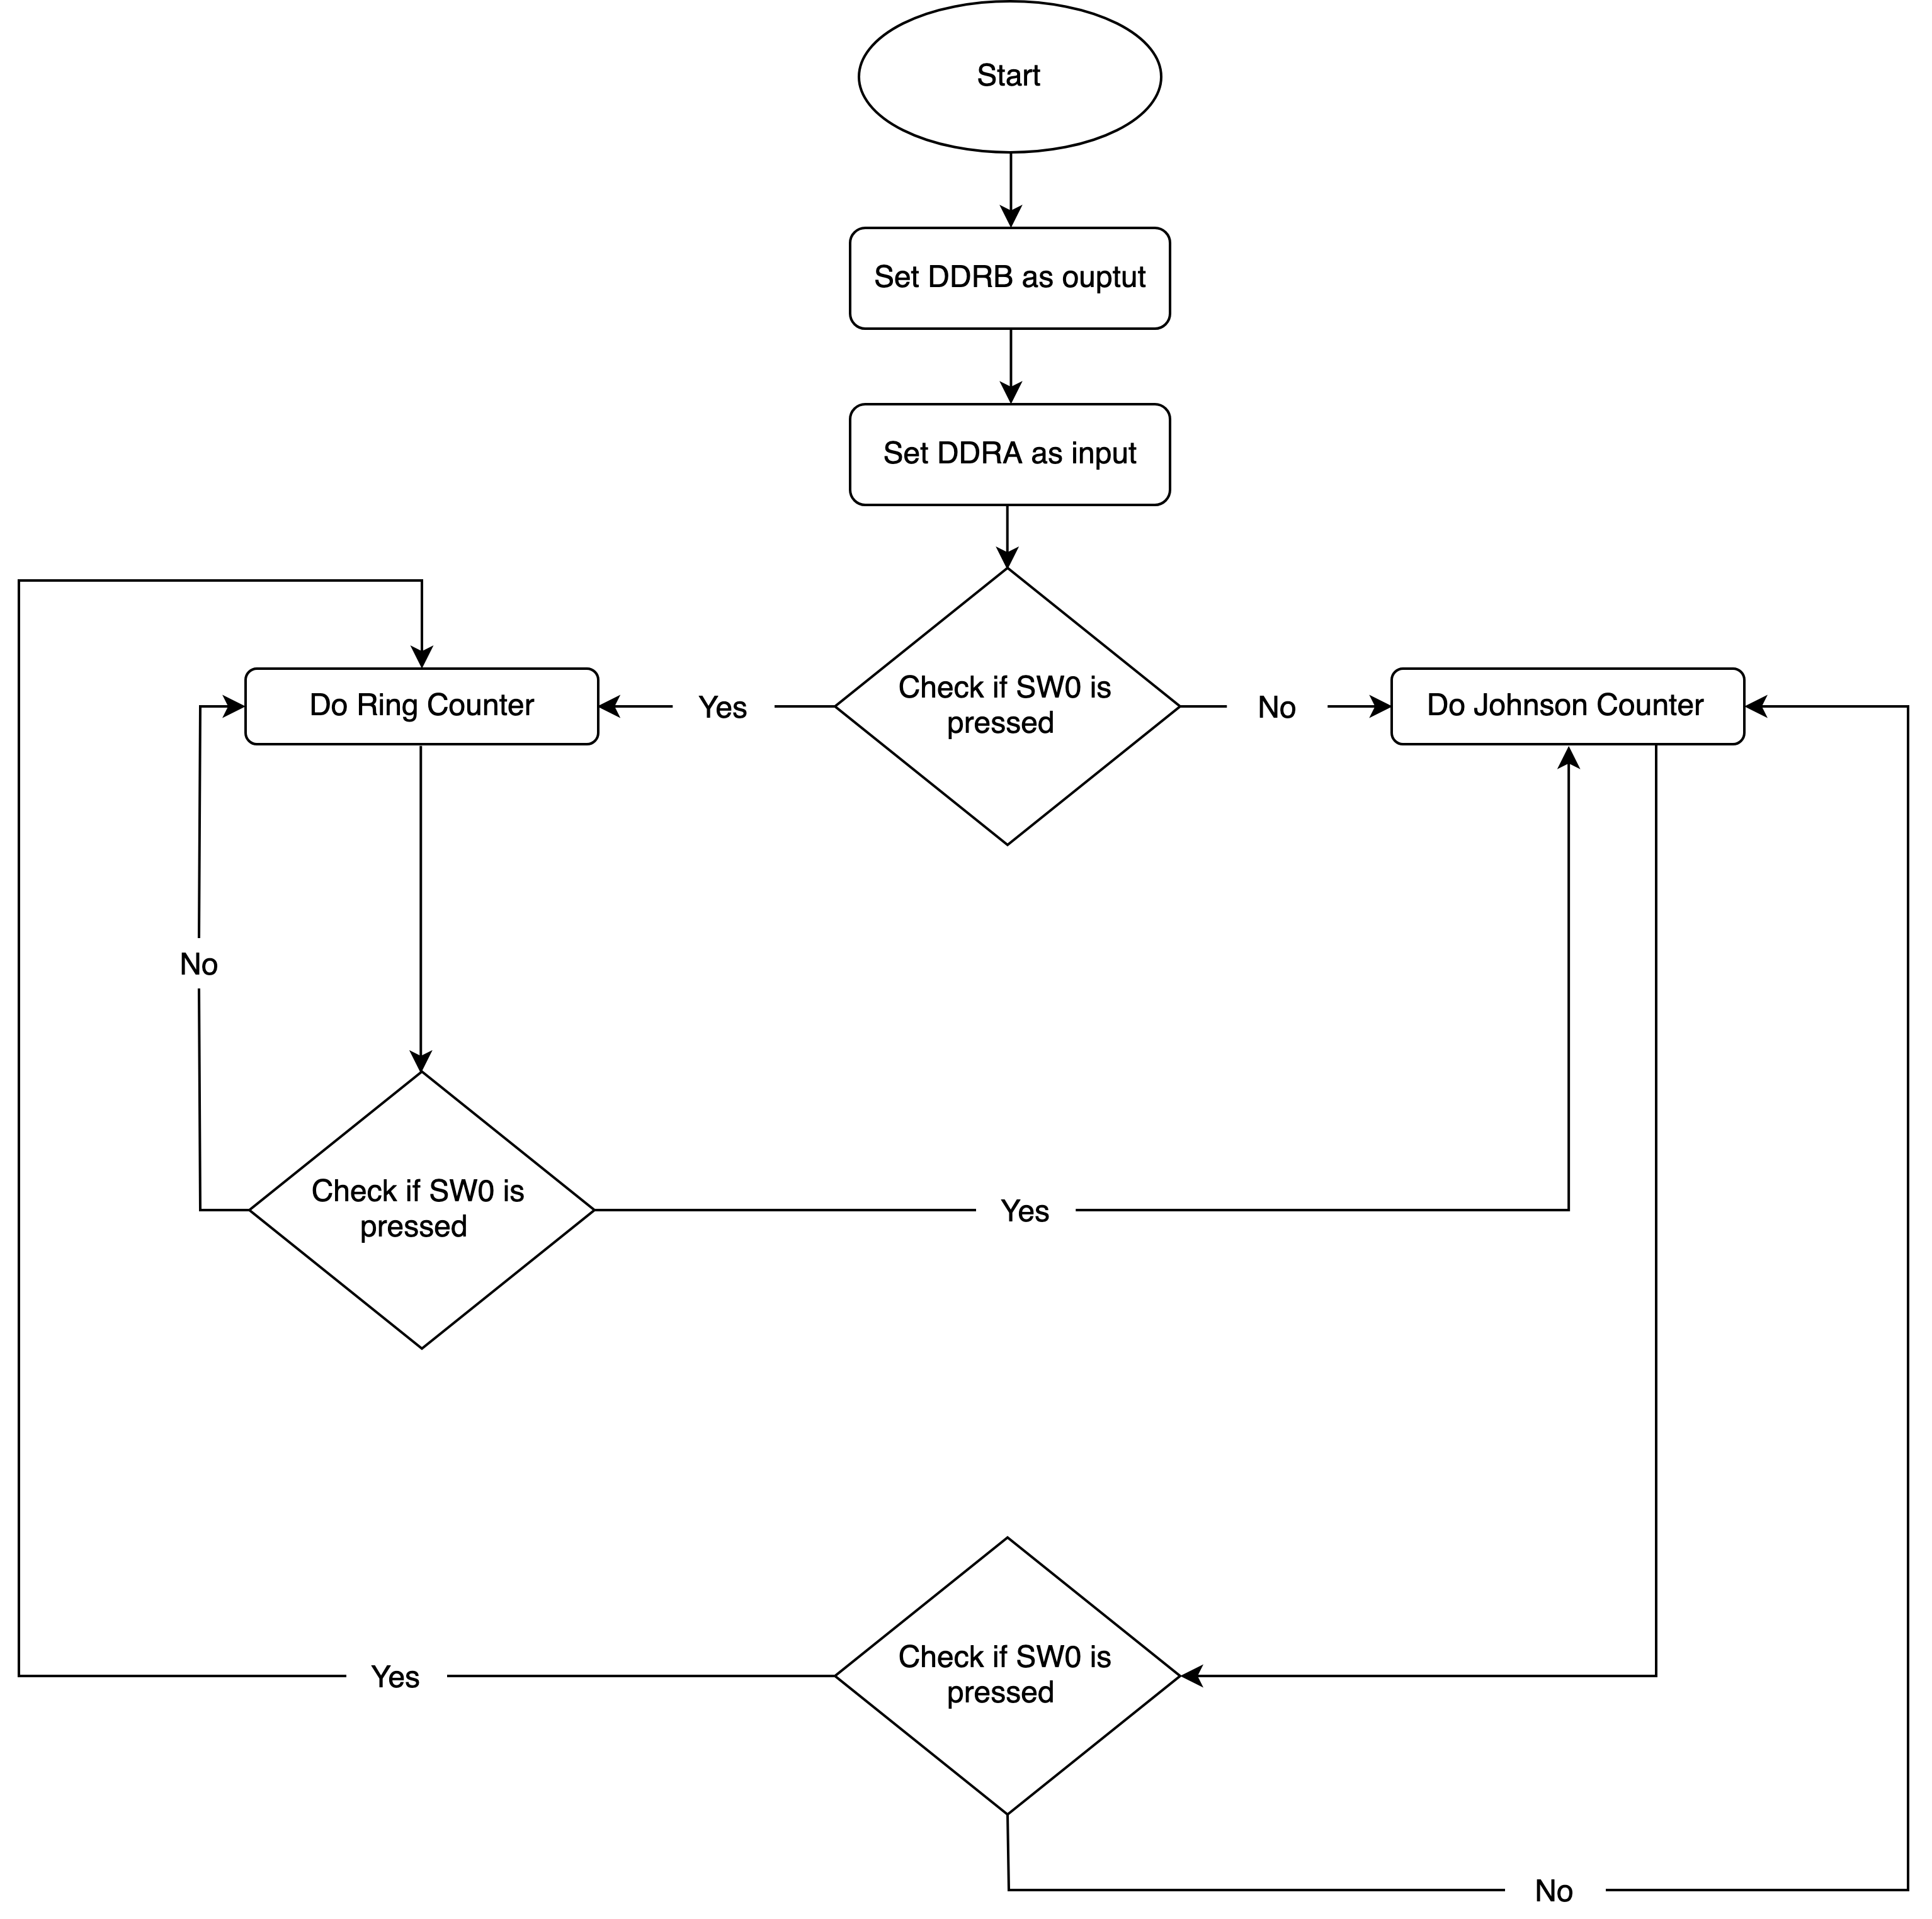
\includegraphics[width=\textwidth/1 ]{flowchart/task1_flowchart.png}
\end{center}
\caption{Task 1 flowchart}
\label{task1}
\end{figure}
\break


%TASK2
\section{Task 2}

\lstset{style=Asm}

\begin{lstlisting}
;>>>>>>>>>>>>>>>>>>>>>>>>>>>>>>>>>>>>>>>>>>>>>>>>>>>>>>>>>>>
; 1DT301, Computer Technology I
; Date: 2016-09-15
; Author:
;	Anas Kwefati
;
; Lab number: 2
; Title: Subroutines
;
; Hardware: STK600, CPU ATmega2560
;
; Function: Create an electronic dice. The number 1 to 6 should be generated randomly. The result should be displayed through the LEDs
;
; Input ports: PORTA checks if we pressed the switch 0 (SW0).
;
; Output ports: PORTB turns on/off the light (LEDs)
;
; Subroutines: If applicable.
; Included files: m2560def.inc
;
; Other information:
;
; Changes in program: (Description and date)
;<<<<<<<<<<<<<<<<<<<<<<<<<<<<<<<<<<<<<<<<<<<<<<<<<<<<<<<<<<<

.include "m2560def.inc"

; Initialize SP, Stack Pointer
ldi r21, HIGH(RAMEND) ; R20 = high part of RAMEND address
out SPH,R21 ; SPH = high part of RAMEND address
ldi R21, low(RAMEND) ; R20 = low part of RAMEND address
out SPL,R21 ; SPL = low part of RAMEND address

;we initialize
ldi r16, 0xFF ; we load 0b1111 1111 to r16
out DDRB, r16 ; we set the DDRB as output

ldi r17, 0x00 ; we load 0b0000 0000 to r17
out DDRA, r17 ; we set DDRA as input


out PORTB, r16 ;we output r16 to PORTB

ldi r18, 0b11111110 ; we load 0b1111 1110 to r18
;it will allow us to make sure that SW0 is pressed

ldi r20, 1 ; we load 0b0000 0001 to r20

ldi r16, 0b11111111 ;we load 0b1111 1111 to r16

loop :
	;We check if SW0 is pressed or not
	in r19,PINA ;we put PINA data into r19
	cp r19, r18 ;we compare r19 to r18 (0b1111 1110)
	breq listening_loop ; if r19 == r18 then go to listening_loop

rjmp loop ;otherwise jump back to loop and repeat it until it is true (SW0 pressed)


listening_loop :
	inc r20 ;we increment r20 by 1
	cpi r20, 7 ;cpi allows us to compare constant numbers.
	;so here compare r20 to 7
	breq reset ;if r20 == 7 we go to reset
	;this part allow us to check if SW0 is still pressed or not.
	;if PINA is still pressed, we stay in this loop and r20 gets +1
	;if it is not pressed anymore, so we released the button we go to random
	in r19, PINA ;we put PINA data into r19
	cp r16,r19 ;we compare r16 (0b1111 1111) and r19
	breq random ; if r16 == r19 we go to random
rjmp listening_loop ;jump back to listening_loop if button SW0 not released

reset :
	ldi r20, 1 ;we set back r10 to 1 when r20 reaches 7
	rjmp loop ;and we jump back to the beginning loop

random :
;this part allows us to do the random process. Meaning, we check the constant
;If the Constant r20 is equal to the corresponding number
; it will go to another section of the program

	cpi r20, 1 ;we compare the constant r19 to check if r20 == 1
	breq number_one ;if yes we go to number_one
	cpi r20, 2
	breq number_two
	cpi r20, 3
	breq number_three
	cpi r20, 4
	breq number_four
	cpi r20, 5
	breq number_five
	cpi r20, 6
	breq number_six


number_one:
	ldi r22, 0b11111101 ;we load 0b1111 1101 to r22
	out PORTB, r22 ;we turn on the light LED 2
	rjmp loop ;we turn on the light and we go back to the loop and wait
	;we wait for another SW0 pressed

number_two:
	ldi r22, 0b10111101
	out PORTB, r22
rjmp loop
number_three:
	ldi r22, 0b10101011
	out PORTB, r22
rjmp loop
number_four:
	ldi r22, 0b00111001
	out PORTB, r22
rjmp loop
number_five:
	ldi r22, 0b00101001
	out PORTB, r22
rjmp loop
number_six:
	ldi r22, 0b00010001
	out PORTB, r22
rjmp loop

\end{lstlisting}

\begin{figure}
\begin{center}
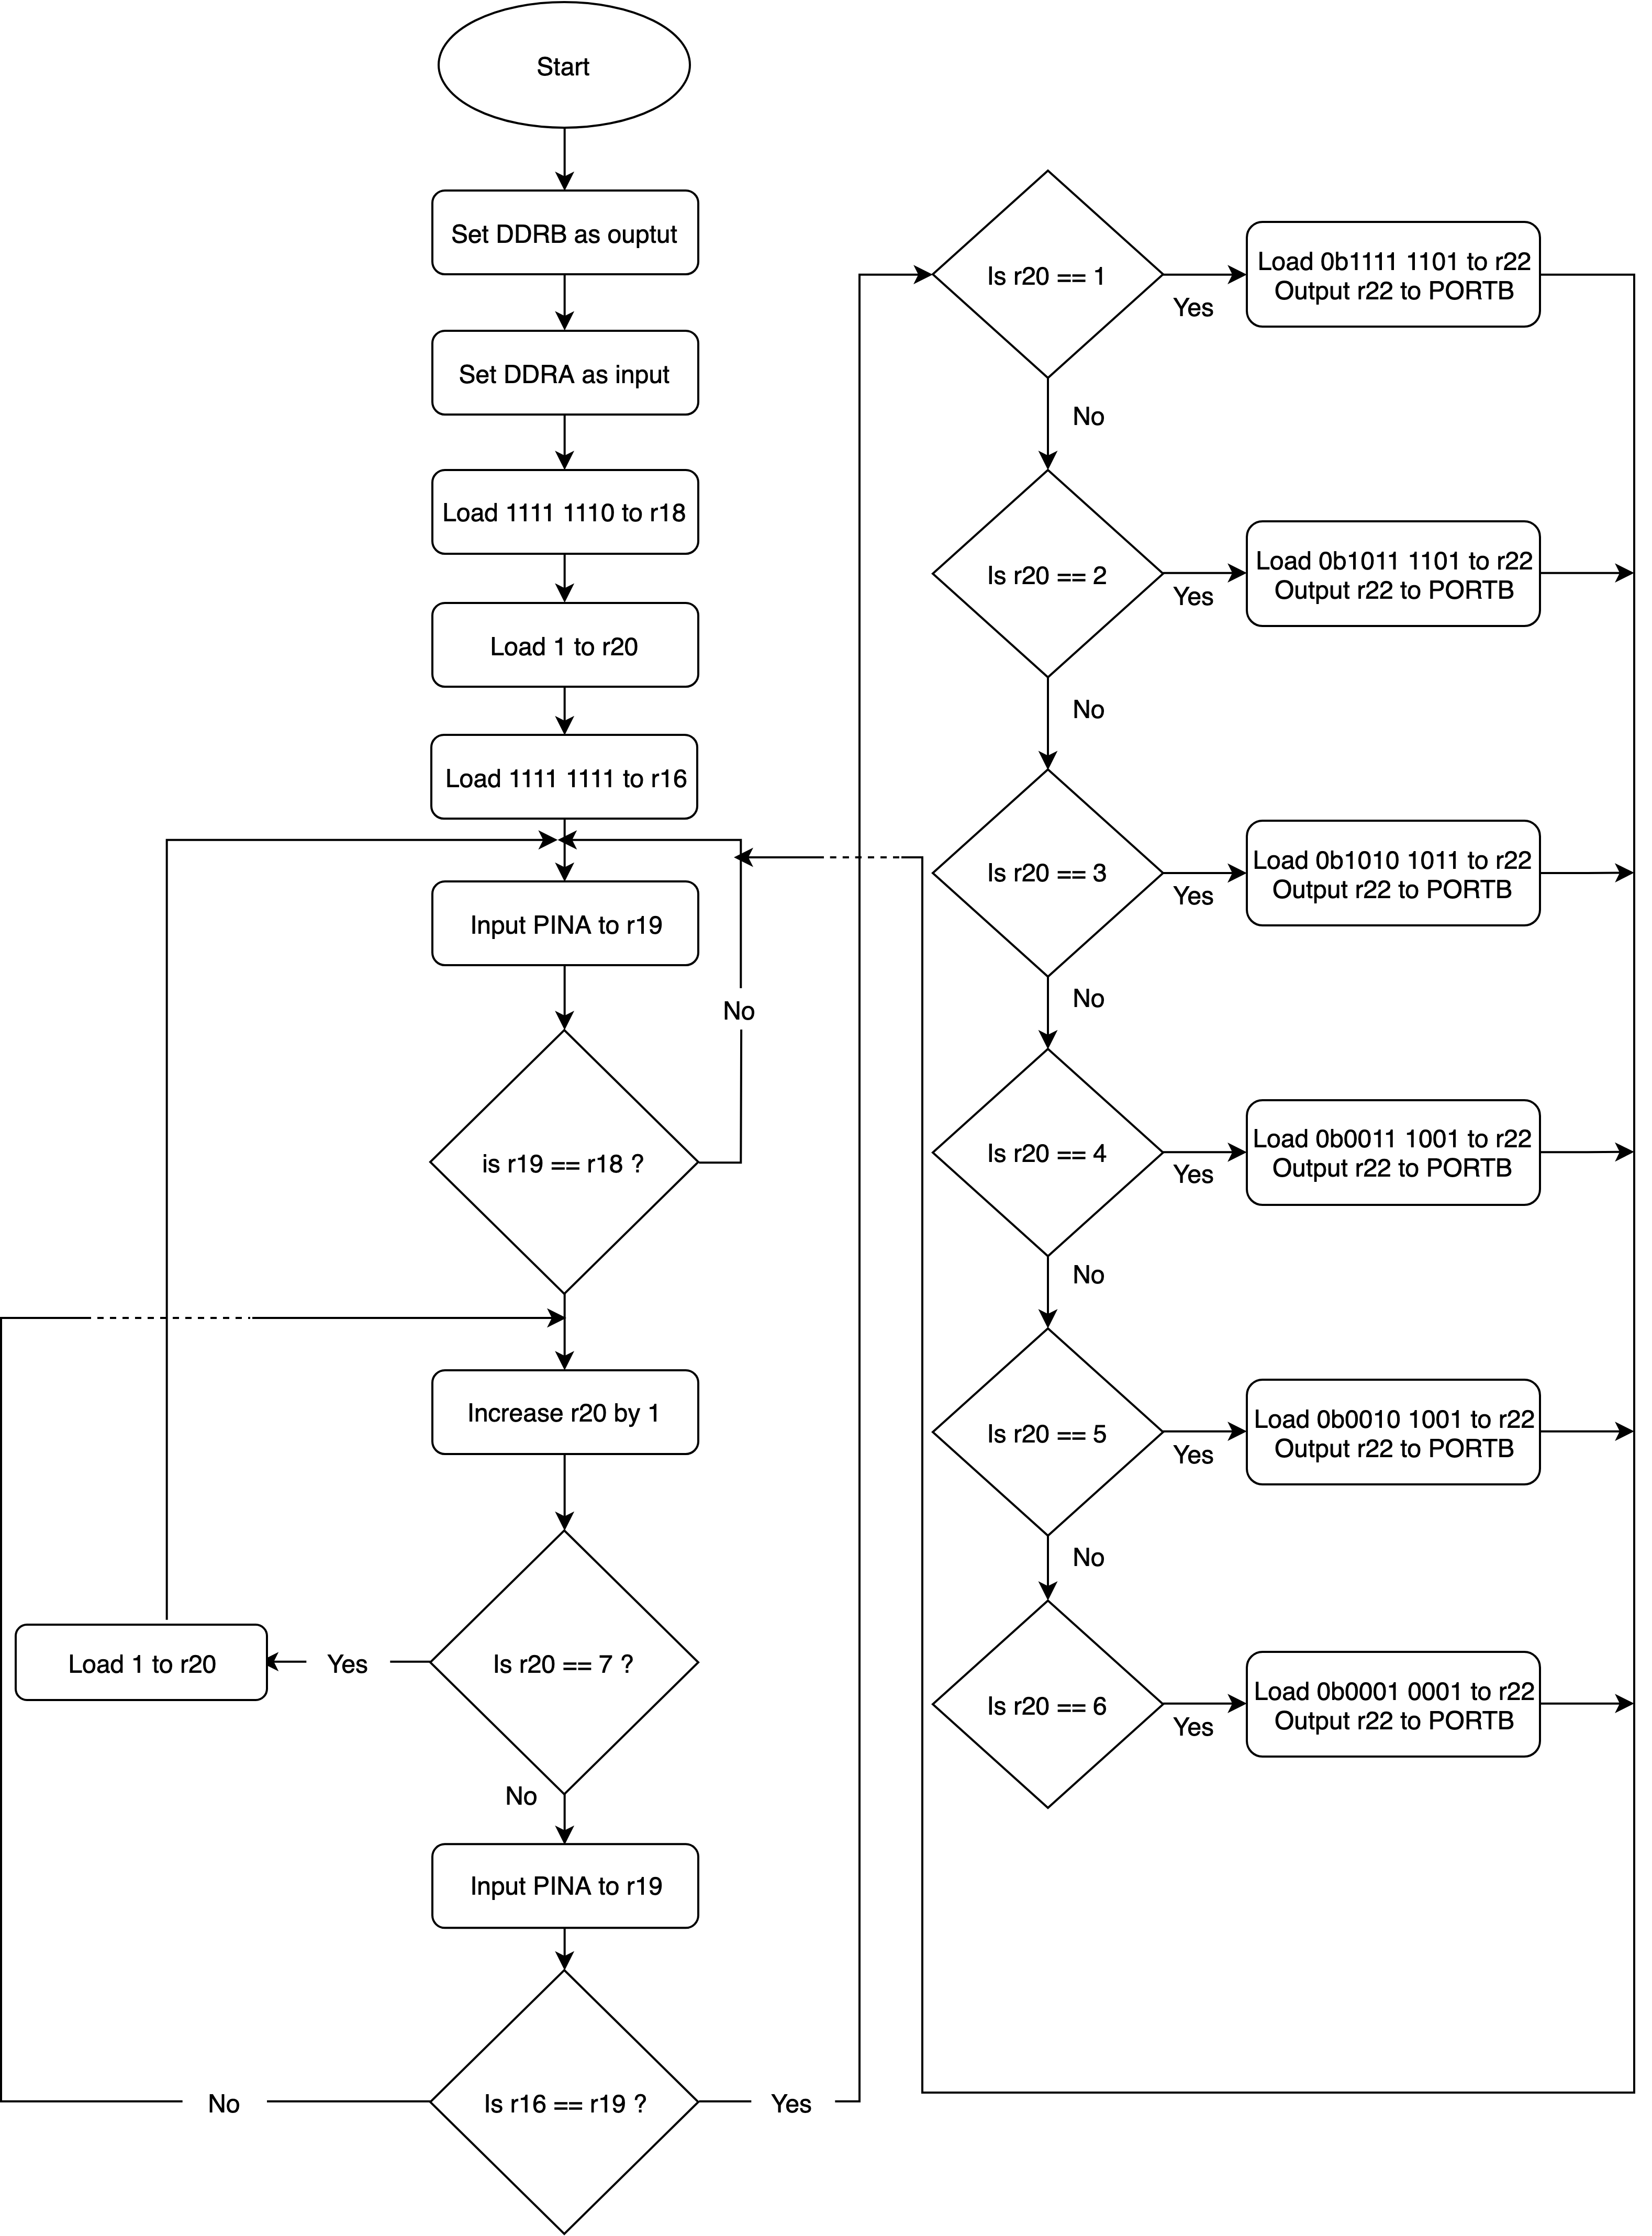
\includegraphics[width=\textwidth/1]{flowchart/task2_flowchart.png}
\end{center}
\caption{Task 2 flowchart}
\label{task2}
\end{figure}

\break

%TASK 3
\section{Task 3}

\lstset{style=Asm}

\begin{lstlisting}
;>>>>>>>>>>>>>>>>>>>>>>>>>>>>>>>>>>>>>>>>>>>>>>>>>>>>>>>>>>>
; 1DT301, Computer Technology I
; Date: 2016-09-15
; Author:
;	Anas Kwefati
;
; Lab number: 2
; Title: Subroutines
;
; Hardware: STK600, CPU ATmega2560
;
; Function: The program counts the number of time we press and release SW0
;
; Input ports: PORTA checks if we pressed the switch 0 (SW0).
;
; Output ports: PORTB turns on/off the light (LEDs)
;
; Subroutines: If applicable.
; Included files: m2560def.inc
;
; Other information:
;
; Changes in program: (Description and date)
;<<<<<<<<<<<<<<<<<<<<<<<<<<<<<<<<<<<<<<<<<<<<<<<<<<<<<<<<<<<
.include "m2560def.inc"

; Initialize SP, Stack Pointer
ldi r21, HIGH(RAMEND) ; R20 = high part of RAMEND address
out SPH,R21 ; SPH = high part of RAMEND address
ldi R21, low(RAMEND) ; R20 = low part of RAMEND address
out SPL,R21 ; SPL = low part of RAMEND address

;we initialize
ldi r16, 0xFF ;
out DDRB, r16 ; we set the DDRB as output

ldi r17, 0x00
out DDRA, r17 ; we set DDRA as input

out PORTB, r16

ldi r18, 0b00000000 ; counter

ldi r19, 0b11111101 ; to check if button is pressed
ldi r23, 0xFF

loop :
	in r20, PINA
	cp r20,r19 ;compare r20 and r19
	breq counting ;if equal then go to counting
rjmp loop


counting :
	inc r18 ; we add +1 to the counter
	;so when we press the first time r18 will become : 0b0000 0001

	mov r21, r18 ; we copy r18 to r21
	com r21 ; we put the reverse of what was in r21.
	
	;0 becomes 1 and 1 becomes 0. We put the complement of r21
	;So here, r21 will become 0b1111 1110
	;we display the binary value. When LEDs are turned on it means 1
	;When LED is not turned on it means 0.
	;For example when we press, we count 1 and its binary value is : 0000 0001
	;We reverse it and we get 1111 1110. Which means we turn on the light at LED1
	;In LED logic, 0 means light on and 1 means light off.
	;When light is on (0 for LED logic) for us it will mean 1.
	;When light is off (1 for LED logic) for us it will mean 0.

	out PORTB, r21 ;we output r21 in PORTB to turn the correct LED position

	counting_loop :

		in r20, PINA ; we take the data of PINA and put it in r20
		cp r20, r23 ; we compare r20 with r23

		breq whatever ;if r20 == r23 we go to whatever

		rjmp counting_loop ;else we go back to the beginning of that loop

whatever :
	inc r18 ;we increment r18 by 1
	mov r21, r18 ;we copy r18 to r21
	com r21 ;  we put the reverse of what was in r21.

	out PORTB, r21 ;we output it in PORTB

	rjmp loop ;we start over, from the beginning
\end{lstlisting}

\begin{figure}
\begin{center}
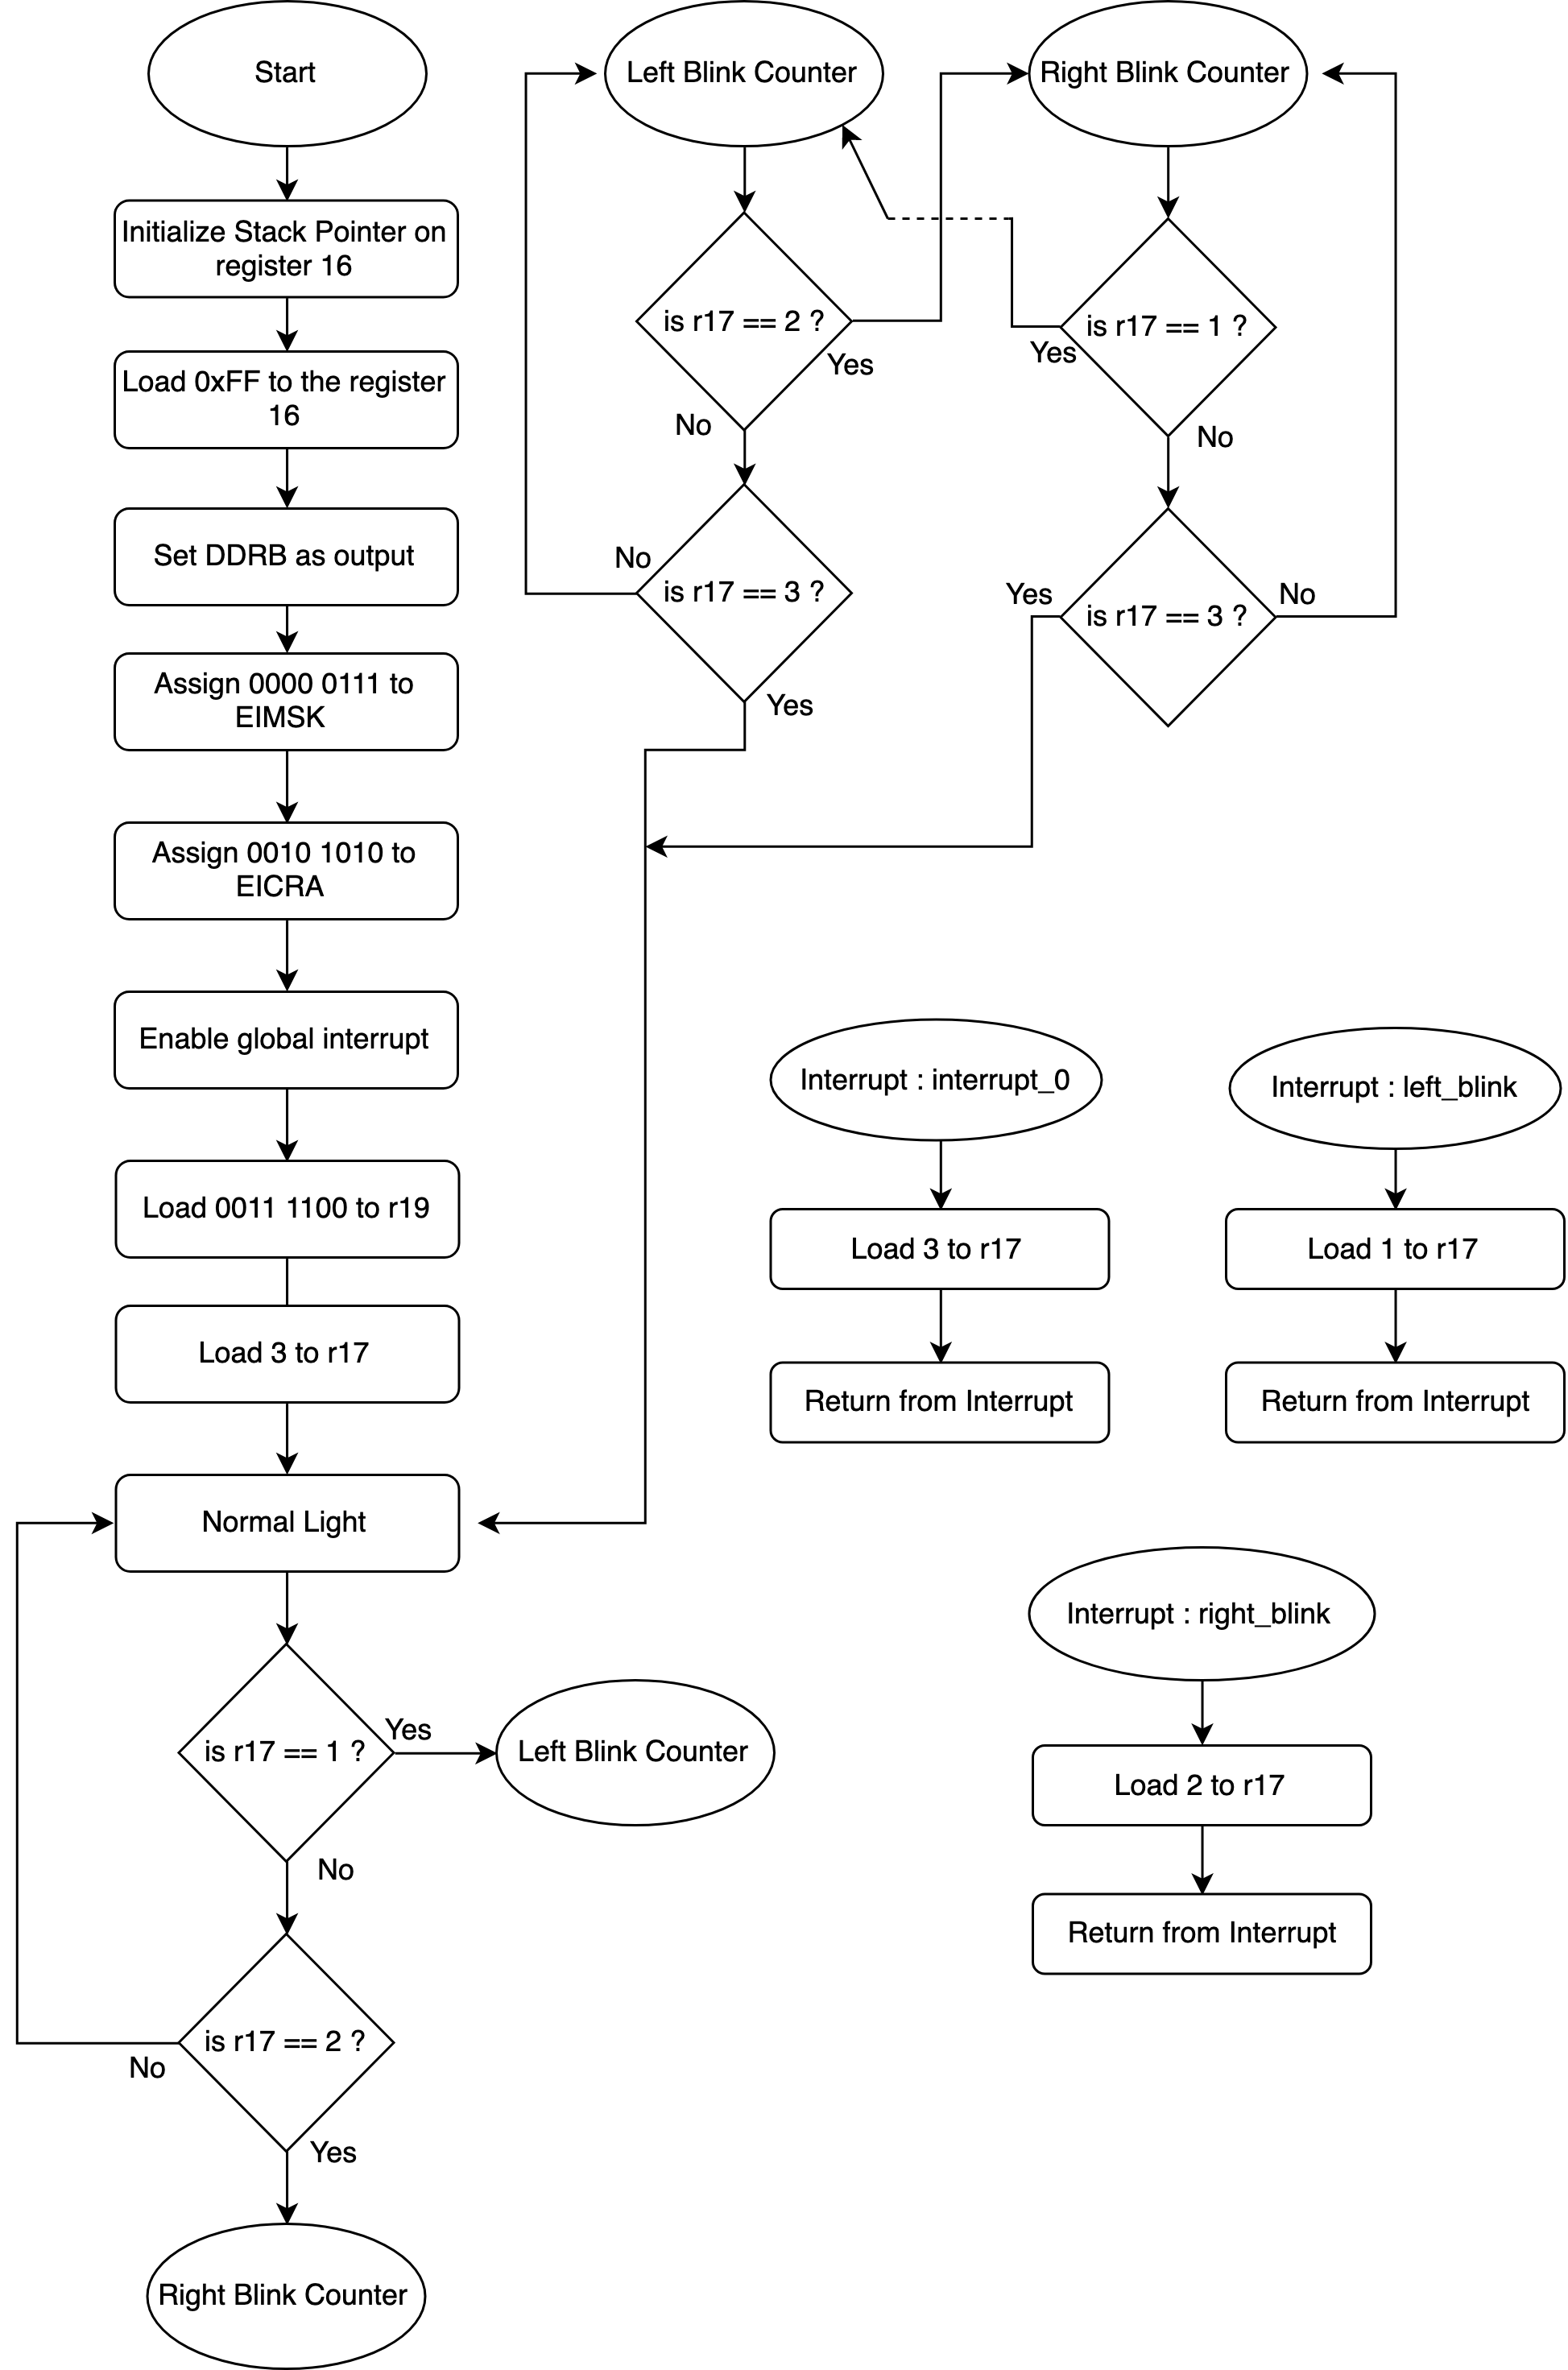
\includegraphics[width=\textwidth/3 ]{flowchart/task3_flowchart.png}
\end{center}
\caption{Task 3 flowchart}
\label{task3}
\end{figure}

\break

%TASK4
\section{Task 4}

\lstset{style=Asm}

\begin{lstlisting}
;>>>>>>>>>>>>>>>>>>>>>>>>>>>>>>>>>>>>>>>>>>>>>>>>>>>>>>>>>>>
; 1DT301, Computer Technology I
; Date: 2016-09-15
; Author:
; Anas Kwefati
;
; Lab number: 2
; Title: Subroutines
;
; Hardware: STK600, CPU ATmega2560
;
; Function: Ring Counter program with a different delay, with a number of ms transferred to
;register pair r25:24
;
; Input ports: None
;
; Output ports: PORTB turns on/off the light (LEDs)
;
; Subroutines: If applicable.
; Included files: m2560def.inc
;
; Other information:
;
; Changes in program: (Description and date)
;<<<<<<<<<<<<<<<<<<<<<<<<<<<<<<<<<<<<<<<<<<<<<<<<<<<<<<<<<<<

.include "m2560def.inc"

; Initialize SP, Stack Pointer
ldi r21, HIGH(RAMEND) ; R20 = high part of RAMEND address
out SPH,R21 ; SPH = high part of RAMEND address
ldi R21, low(RAMEND) ; R20 = low part of RAMEND address
out SPL,R21 ; SPL = low part of RAMEND address

.equ nbrExecution = 2000 ; equ assigns a constant value to a label therefore this value cannot be changed later
; we define the number of loop executions as constant

;we initialize
ldi r16, 0xFF ;
out DDRB, r16 ; we set the DDRB as output

ring_counter:
	ldi r18, 0b11111110

ring_loop:
	out PORTB, r18 ;we put the value of r18 to PORTB which should turn on the light
	call Delay
	com r18
	LSL r18
	com r18

	;Check if everything is off if true then go to ring counter to make infinite loop
	ldi r21,0xFF
	cp r21, r18
	breq ring_counter
	rjmp ring_loop

Delay :

	; r25:r24 is a 16 bit register and so can have 65,536 different numbers, it can count 256 times longer than with an 8 bit register only.

	;The lower byte of the 16-bit-adress is located in the lower register, the higher byte in the upper register. Both parts have their own names, e.g. the higher byte of Z is named ZH (=R31), the lower Byte is ZL (=R30).
	;These names are defined in the standard header file for the chips. Dividing these 16-bit-pointer-names into two different bytes is done like follows:
	ldi r25, HIGH(nbrExecution) ; We load the Most Significant Bit register with the upper byte from the address nbrExecution
	ldi r24, LOW(nbrExecution) ; We set the Least Significant Bit register with the lower byte from the address nbrExecution

	wait_milliseconds :
		rcall sub_delay ;we call the sub_delay that contains 1ms that is going to be repeated 1000 times to do 1s
		sbiw r24, 1 ; By doing that we substract 1 from the register pair r25:r24
		;We decrease the double register value by 1
		;The instruction "SBIW R24,1" decreases the register pair word-wise. That means that whenever the LSB (Least Significant Bit r24) underflows, the MSB(Most Significant Bit r25) is also automatically reduced by 1.
		brne wait_milliseconds ; if not zero start loop again, if zero continue

sub_delay :
	; Generated by delay loop calculator
	; at http://www.bretmulvey.com/avrdelay.html
	;
	; Delay 2 000 cycles
	; 500us at 4.0 MHz

		ldi  r17, 3
		ldi  r19, 152
	L1: dec  r19
		brne L1
		dec  r17
		brne L1
		nop
		ret
\end{lstlisting}
\break
\begin{figure}
\begin{center}
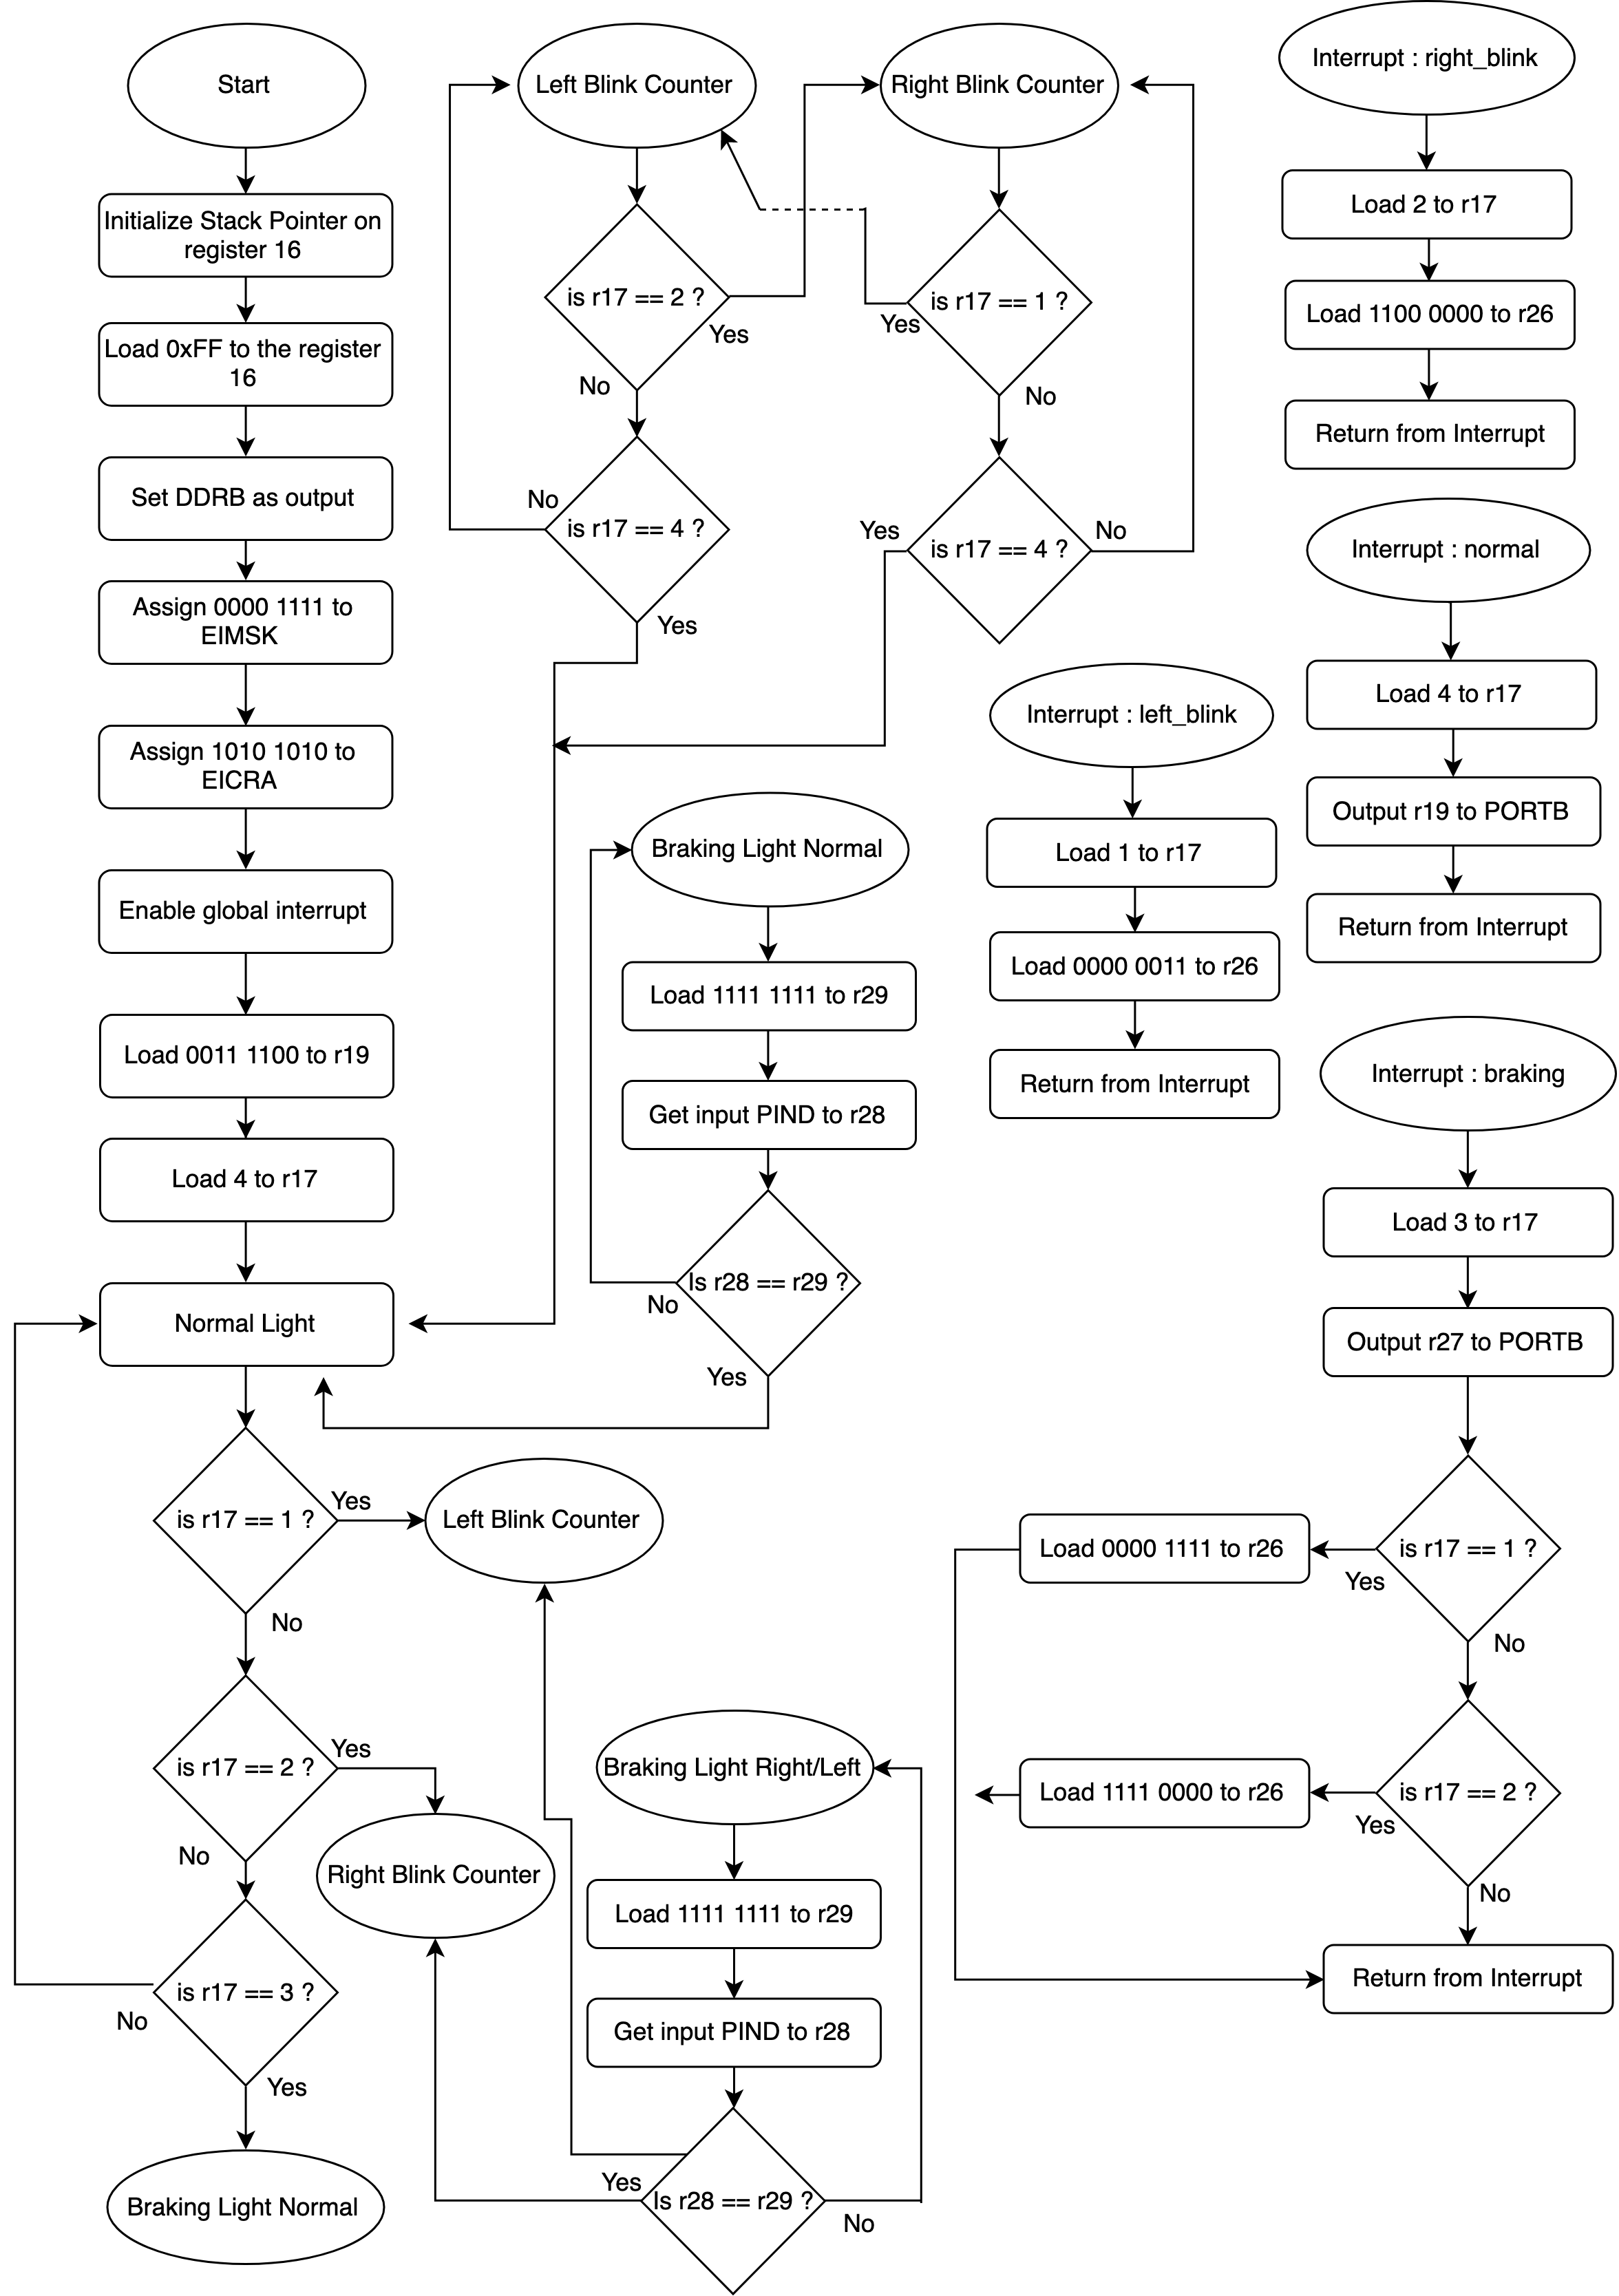
\includegraphics[width=\textwidth/1 ]{flowchart/task4_flowchart.png}
\end{center}
\caption{Task 4 flowchart}
\label{task4}
\end{figure}

\break 

% Prints your bibliography database xxx.bib
\bibliographystyle{IEEEtran}
\bibliography{ref.bib}

\end{document}
